
\subsection{Experimentation}
\begin{frame}
  
  Different random instances were created,
  Some results are shown graphically
  \begin{center}
    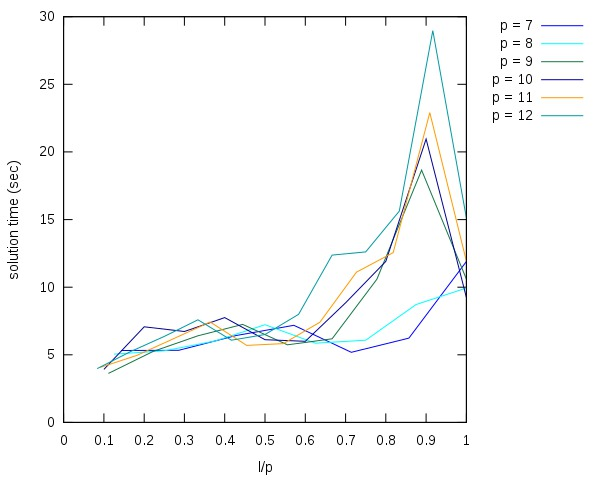
\includegraphics[scale=0.25]{grafica_01}
    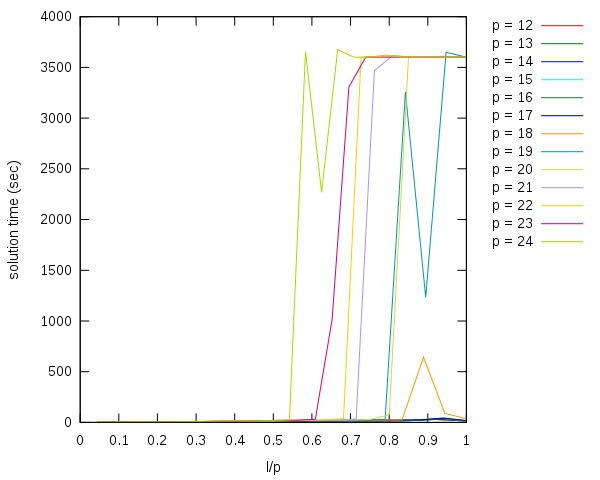
\includegraphics[scale=0.25]{grafica_02}
  \end{center}
\end{frame}

\begin{frame}

  The times for some values of \textit{l} in relation with \textit{p} 
  increase drastically
  \begin{center}
    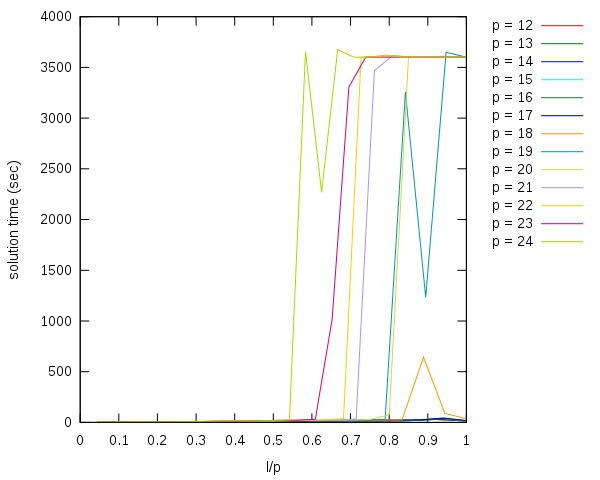
\includegraphics[scale=0.25]{grafica_02}
    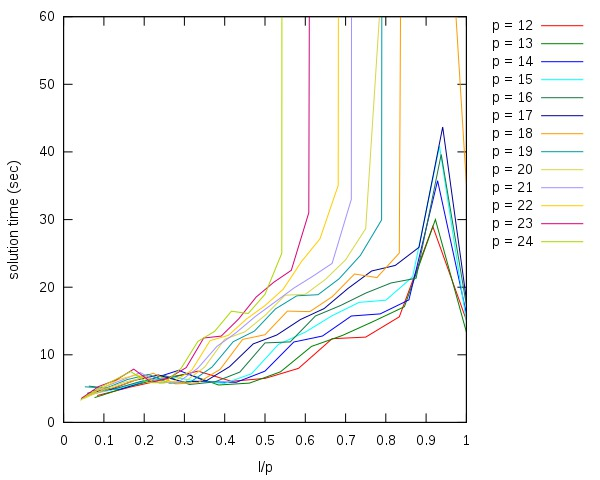
\includegraphics[scale=0.25]{grafica_03}
  \end{center}
  
\end{frame}

\begin{frame}

  But the results for small values of \textit{l},
  they remain in effect for the rest of the instances.
  \begin{center}
    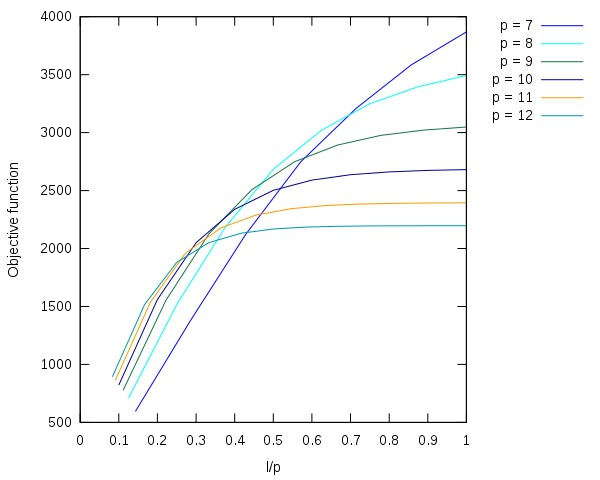
\includegraphics[scale=0.25]{grafica_04}
    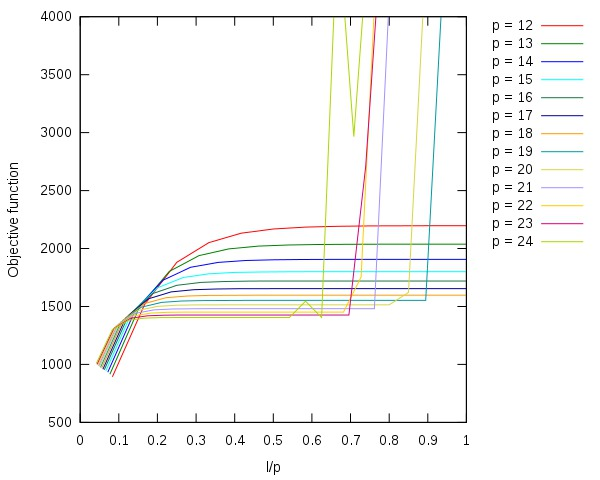
\includegraphics[scale=0.25]{grafica_05}
  \end{center}
  
\end{frame}

%% Caso 100 30 12
\frame{\begin{figure}[h!]\centering{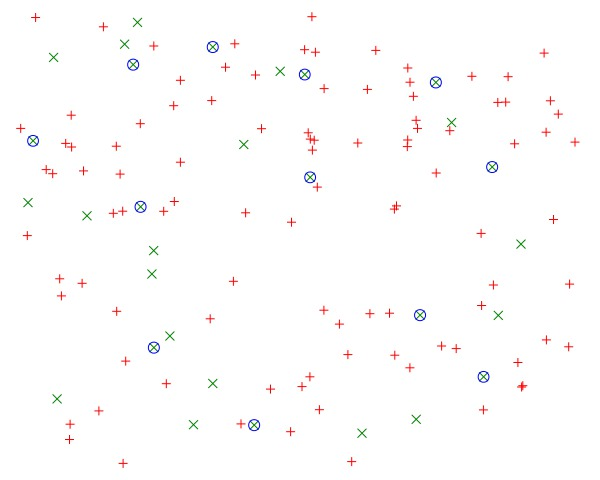
\includegraphics[scale=0.35]{Test_100_30_12_01}\caption{n = 100, m = 30, p = 12, l = 1}}\end{figure}}
\frame{\begin{figure}[h!]\centering{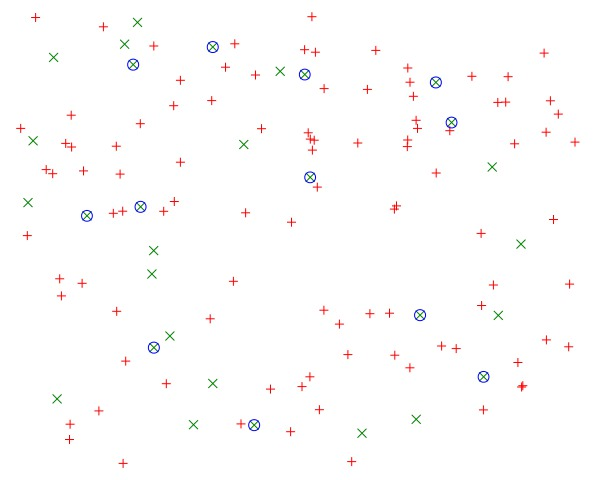
\includegraphics[scale=0.35]{Test_100_30_12_02}\caption{n = 100, m = 30, p = 12, l = 2}}\end{figure}}
\frame{\begin{figure}[h!]\centering{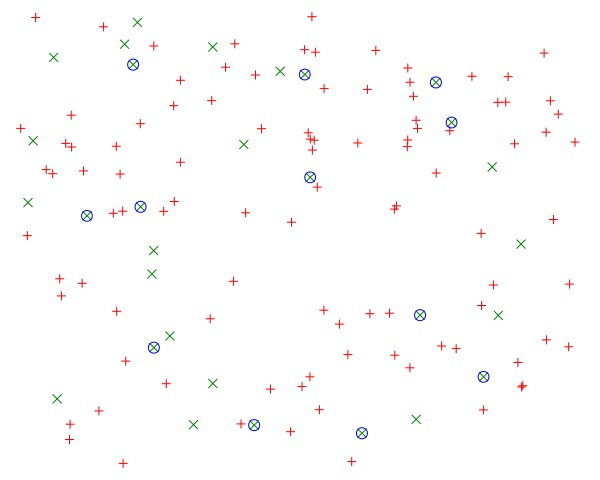
\includegraphics[scale=0.35]{Test_100_30_12_03}\caption{n = 100, m = 30, p = 12, l = 3}}\end{figure}}
\frame{\begin{figure}[h!]\centering{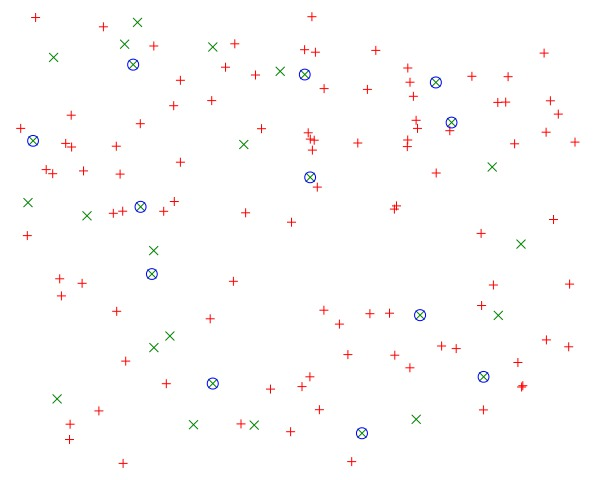
\includegraphics[scale=0.35]{Test_100_30_12_04}\caption{n = 100, m = 30, p = 12, l = 4}}\end{figure}}
\frame{\begin{figure}[h!]\centering{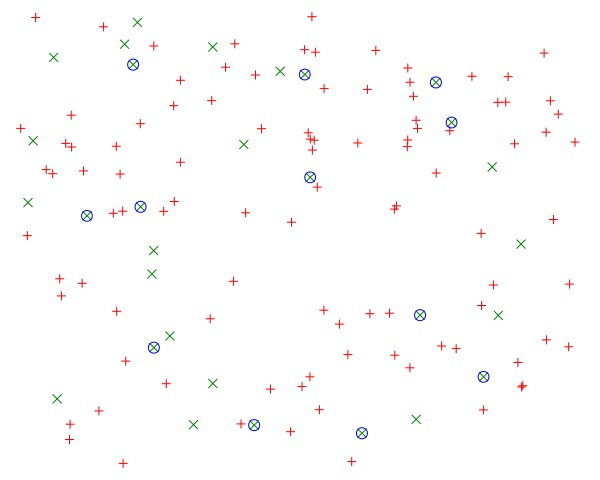
\includegraphics[scale=0.35]{Test_100_30_12_05}\caption{n = 100, m = 30, p = 12, l = 5}}\end{figure}}
\frame{\begin{figure}[h!]\centering{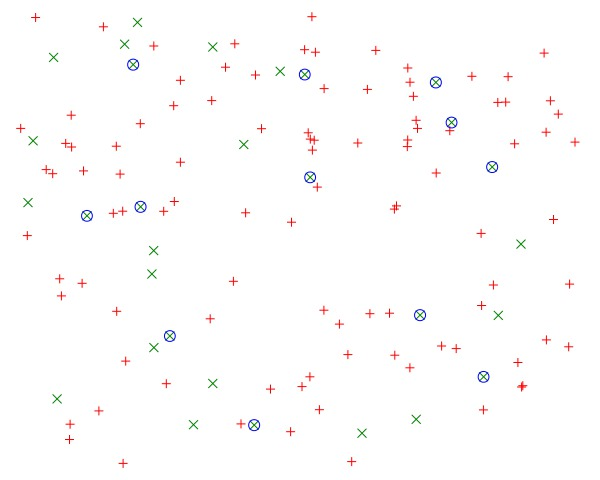
\includegraphics[scale=0.35]{Test_100_30_12_06}\caption{n = 100, m = 30, p = 12, l = 6}}\end{figure}}
\frame{\begin{figure}[h!]\centering{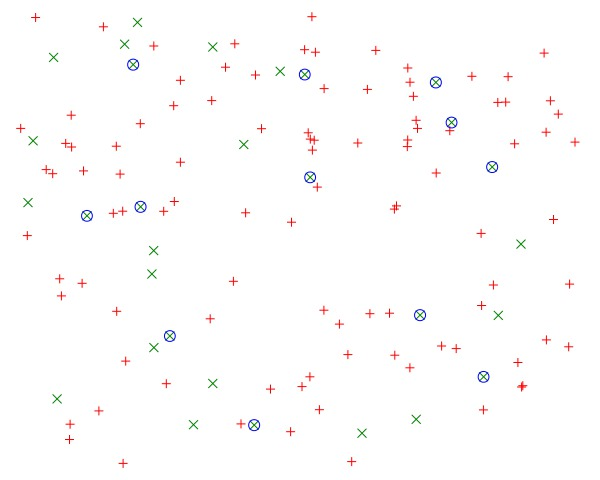
\includegraphics[scale=0.35]{Test_100_30_12_07}\caption{n = 100, m = 30, p = 12, l = 7}}\end{figure}}
\frame{\begin{figure}[h!]\centering{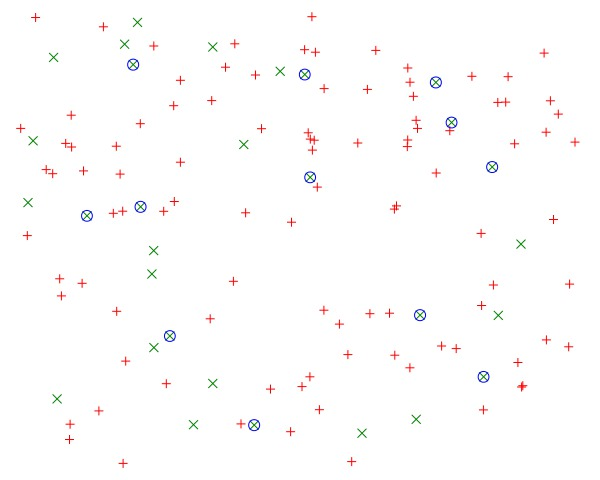
\includegraphics[scale=0.35]{Test_100_30_12_08}\caption{n = 100, m = 30, p = 12, l = 8}}\end{figure}}
\frame{\begin{figure}[h!]\centering{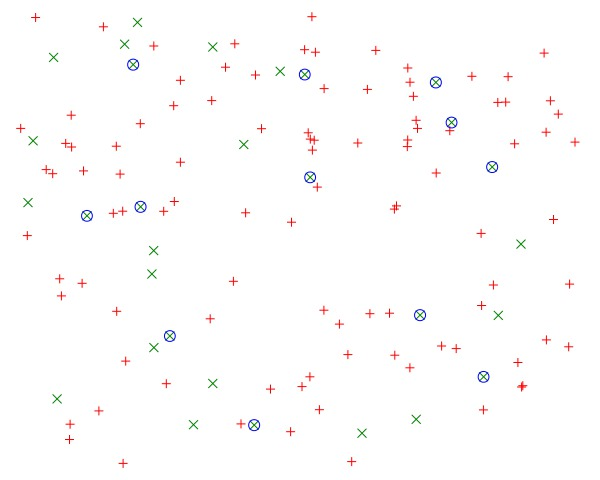
\includegraphics[scale=0.35]{Test_100_30_12_09}\caption{n = 100, m = 30, p = 12, l = 9}}\end{figure}}
\frame{\begin{figure}[h!]\centering{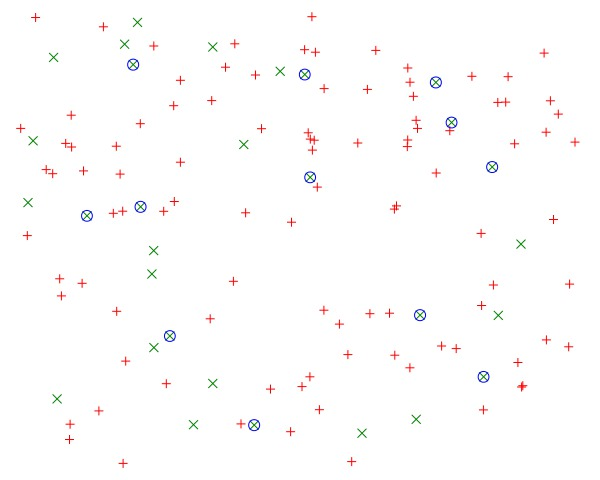
\includegraphics[scale=0.35]{Test_100_30_12_10}\caption{n = 100, m = 30, p = 12, l = 10}}\end{figure}}
\frame{\begin{figure}[h!]\centering{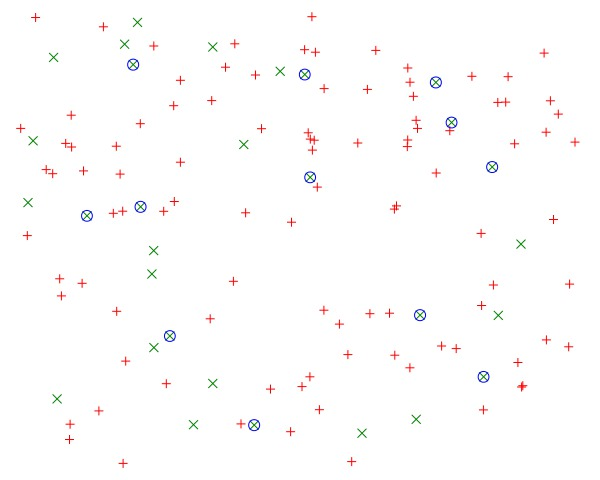
\includegraphics[scale=0.35]{Test_100_30_12_11}\caption{n = 100, m = 30, p = 12, l = 11}}\end{figure}}
\frame{\begin{figure}[h!]\centering{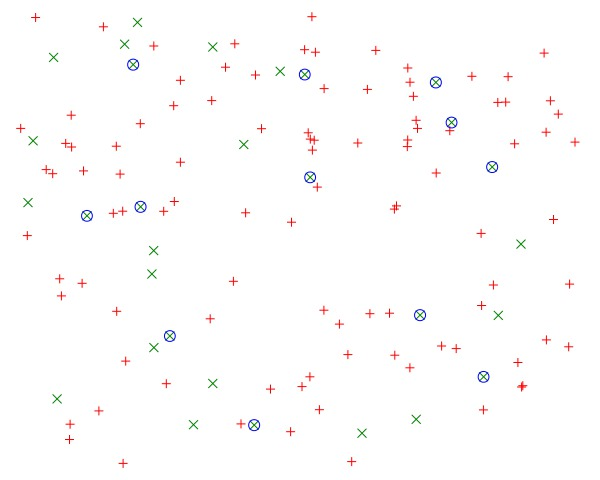
\includegraphics[scale=0.35]{Test_100_30_12_12}\caption{n = 100, m = 30, p = 12, l = 12}}\end{figure}}

\frame{\begin{figure}[h!]\centering{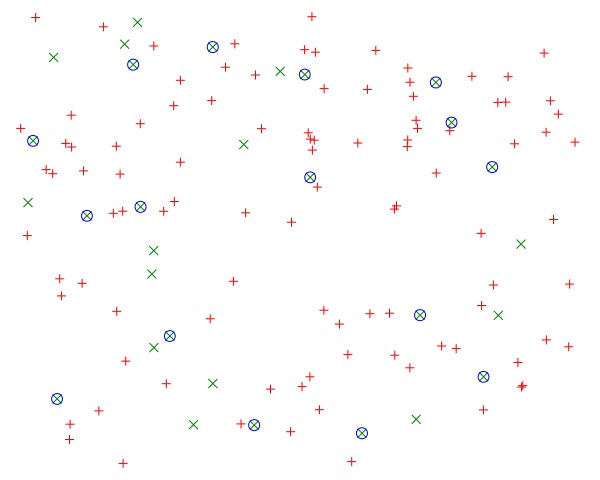
\includegraphics[scale=0.35]{Test_100_30_16_01}\caption{n = 100, m = 30, p = 16, l = 1}}\end{figure}}
\frame{\begin{figure}[h!]\centering{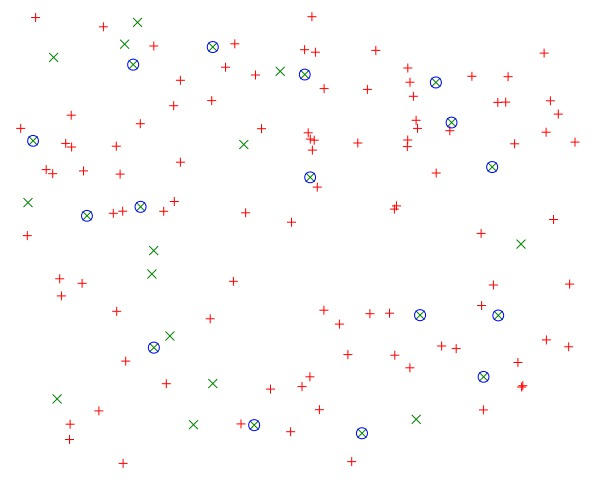
\includegraphics[scale=0.35]{Test_100_30_16_02}\caption{n = 100, m = 30, p = 16, l = 2}}\end{figure}}
\frame{\begin{figure}[h!]\centering{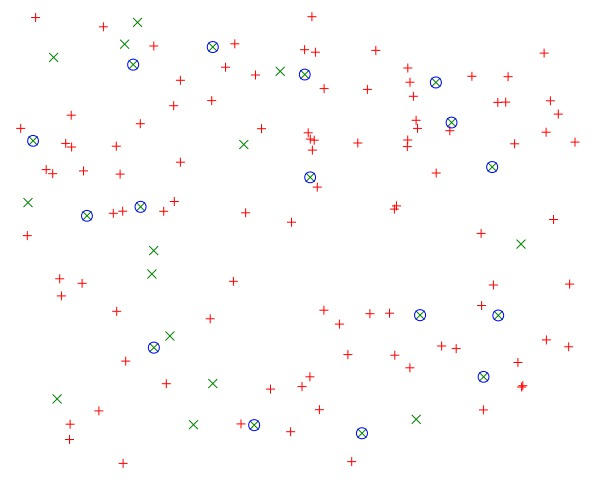
\includegraphics[scale=0.35]{Test_100_30_16_03}\caption{n = 100, m = 30, p = 16, l = 3}}\end{figure}}
\frame{\begin{figure}[h!]\centering{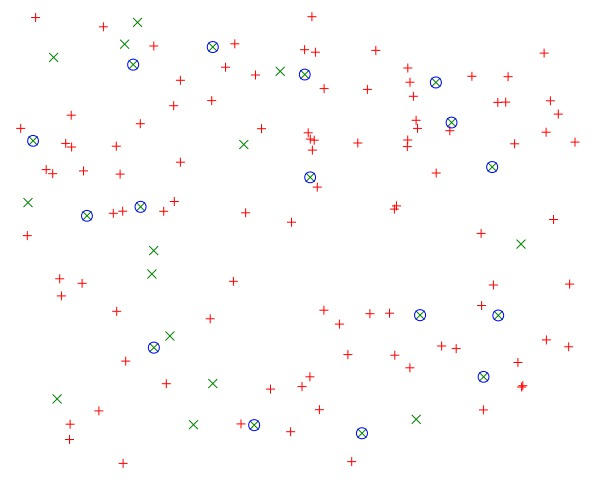
\includegraphics[scale=0.35]{Test_100_30_16_04}\caption{n = 100, m = 30, p = 16, l = 4}}\end{figure}}
\frame{\begin{figure}[h!]\centering{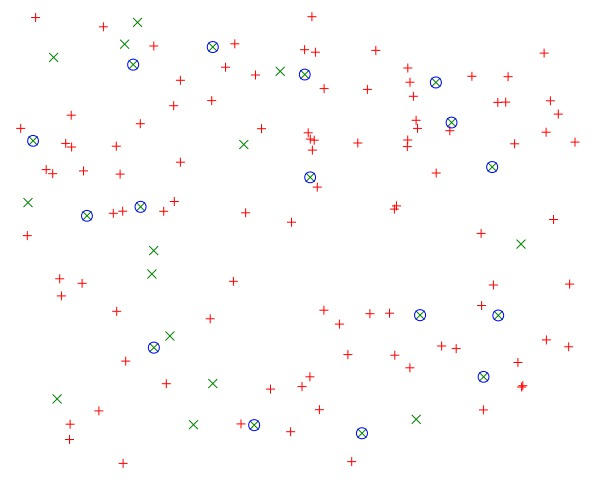
\includegraphics[scale=0.35]{Test_100_30_16_05}\caption{n = 100, m = 30, p = 16, l = 5}}\end{figure}}
\frame{\begin{figure}[h!]\centering{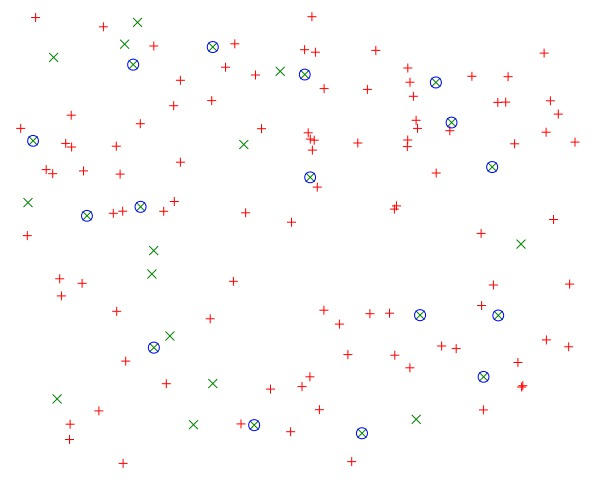
\includegraphics[scale=0.35]{Test_100_30_16_06}\caption{n = 100, m = 30, p = 16, l = 6}}\end{figure}}
\frame{\begin{figure}[h!]\centering{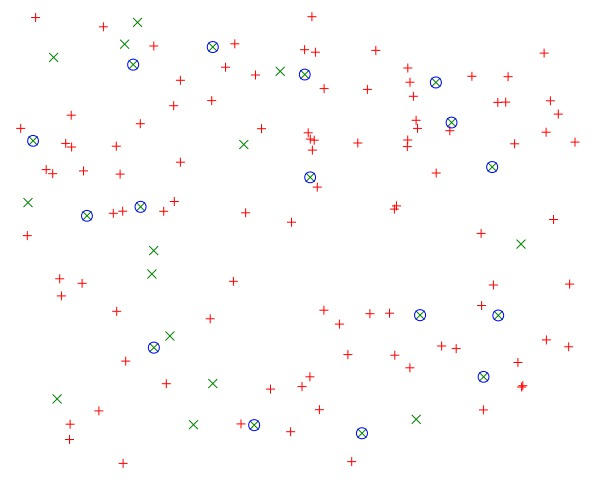
\includegraphics[scale=0.35]{Test_100_30_16_07}\caption{n = 100, m = 30, p = 16, l = 7}}\end{figure}}
\frame{\begin{figure}[h!]\centering{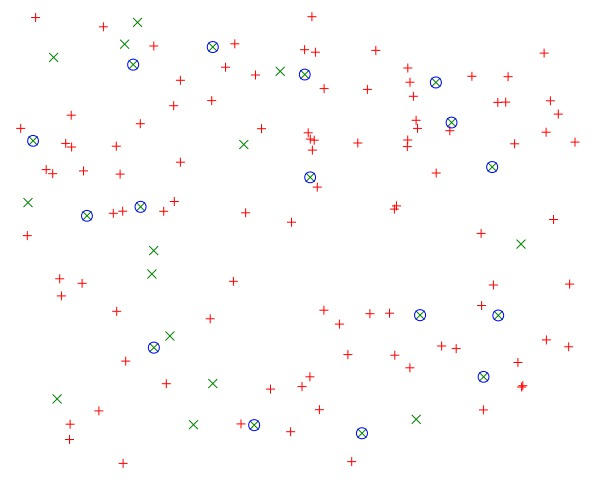
\includegraphics[scale=0.35]{Test_100_30_16_08}\caption{n = 100, m = 30, p = 16, l = 8}}\end{figure}}
\frame{\begin{figure}[h!]\centering{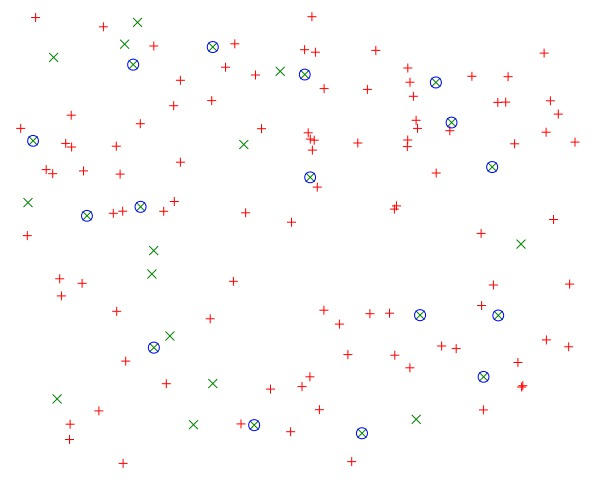
\includegraphics[scale=0.35]{Test_100_30_16_09}\caption{n = 100, m = 30, p = 16, l = 9}}\end{figure}}
\frame{\begin{figure}[h!]\centering{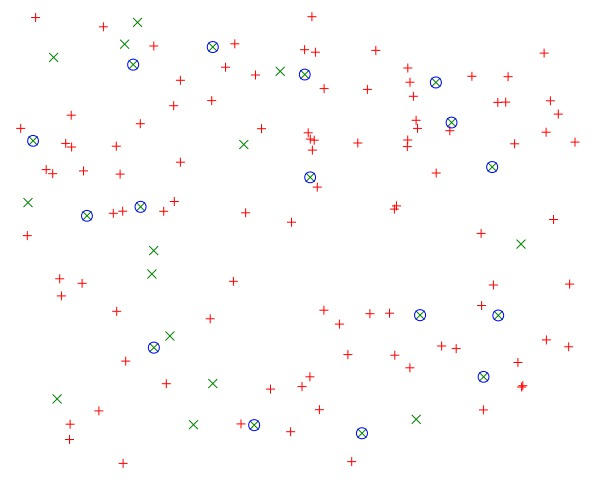
\includegraphics[scale=0.35]{Test_100_30_16_10}\caption{n = 100, m = 30, p = 16, l = 10}}\end{figure}}
\frame{\begin{figure}[h!]\centering{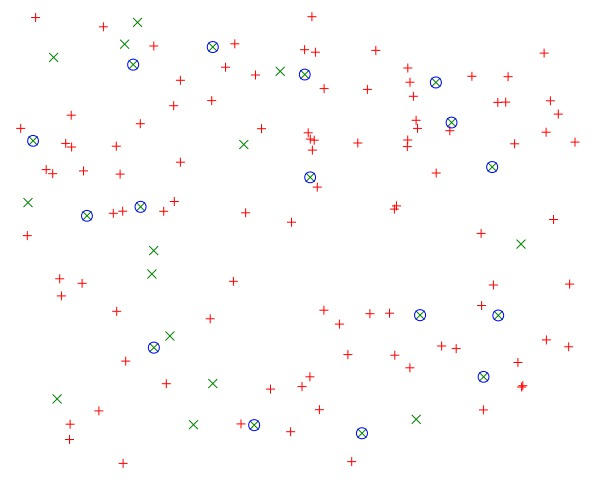
\includegraphics[scale=0.35]{Test_100_30_16_11}\caption{n = 100, m = 30, p = 16, l = 11}}\end{figure}}
\frame{\begin{figure}[h!]\centering{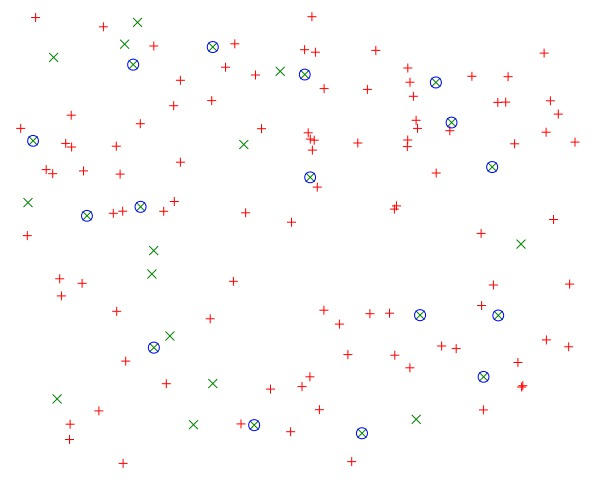
\includegraphics[scale=0.35]{Test_100_30_16_12}\caption{n = 100, m = 30, p = 16, l = 12}}\end{figure}}
\frame{\begin{figure}[h!]\centering{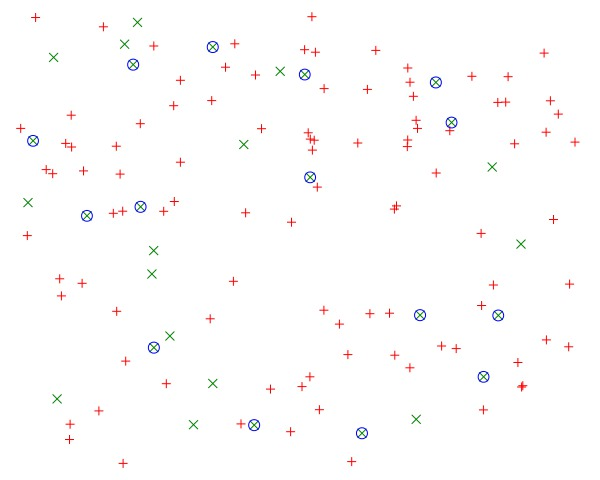
\includegraphics[scale=0.35]{Test_100_30_16_13}\caption{n = 100, m = 30, p = 16, l = 13}}\end{figure}}
\frame{\begin{figure}[h!]\centering{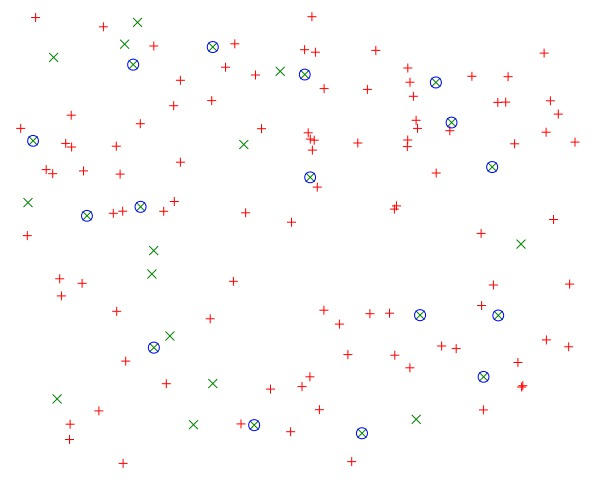
\includegraphics[scale=0.35]{Test_100_30_16_14}\caption{n = 100, m = 30, p = 16, l = 14}}\end{figure}}
\frame{\begin{figure}[h!]\centering{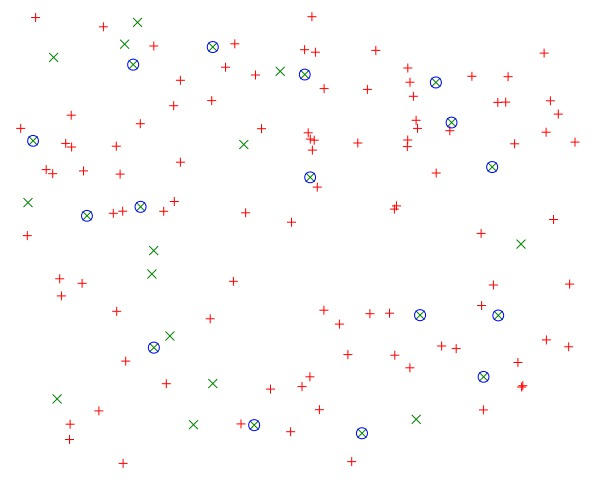
\includegraphics[scale=0.35]{Test_100_30_16_15}\caption{n = 100, m = 30, p = 16, l = 15}}\end{figure}}
\frame{\begin{figure}[h!]\centering{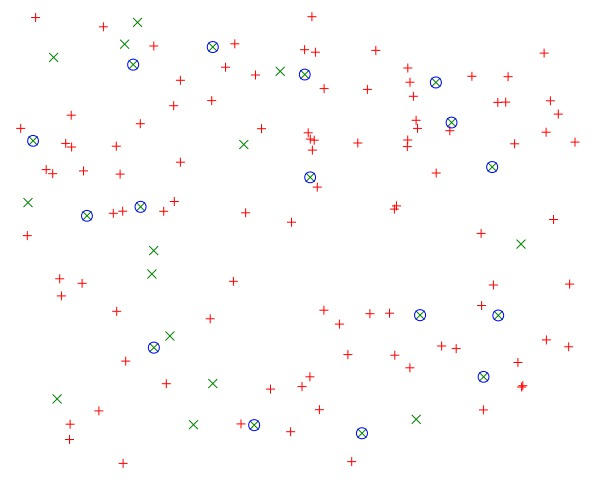
\includegraphics[scale=0.35]{Test_100_30_16_16}\caption{n = 100, m = 30, p = 16, l = 16}}\end{figure}}
